% !TeX root = ../paper.tex
% !TeX encoding = UTF-8
% !TeX spellcheck = en_US

\section{Actor Memory Overhead Experiments}\label{sec:experiments}

  Our concept is based on the usage of hundreds of thousands of \glspl{dactor}, which all store only a small amount of data.
  This raises the question of how much memory overhead is introduced for storing data split across a multitude of actors.
  Therefore, we performed experiments comparing the memory usage of an exemplary actor database system with that of just loading the data into our data storage abstraction, called relations, or in a big string into memory.

\subsection{Experiment Setup}

  \begin{table}
    \centering
    \begin{tabular}{lrrr}
      \toprule
      \textbf{Dataset} & \textbf{Size on disk} & \textbf{\# \glspl{dactor}} & \textbf{\# Relations}\\
      \midrule
      $D_1$ & 10~M & 829 & 1~714 \\
      $D_2$ & 25~M & 2~578 & 5~250 \\
      $D_3$ & 50~M & 4~373 & 8~935 \\
      $D_4$ & 100~M & 8~618 & 17~596 \\
      \bottomrule
    \end{tabular}
    \caption{Datasets used for the memory overhead experiments}
    \label{tab:datasets}
  \end{table}

\subsection{Results}

  \begin{figure}
    \centering
    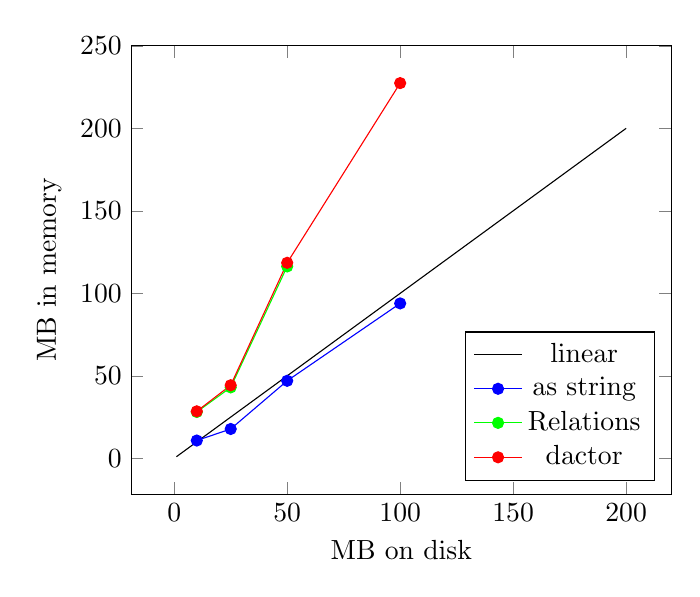
\begin{tikzpicture}
      \begin{axis}[
          xlabel=MB on disk, ylabel=MB in memory,
          legend pos=south east
      ]
        \addplot[mark={}, color=black] coordinates {
          (1,1)
          (200,200)
        };
        \addplot[mark=*, color=blue] coordinates {
          (10,10.8)
          (25,17.8)
          (50,47.0)
          (100,93.9)
        };
        \addplot[mark=*, color=green] coordinates {
          (10,28.1)
          (25,43.0)
          (50,116.3)
        };
        \addplot[mark=*, color=red] coordinates {
          (10,28.5)
          (25,44.3)
          (50,118.5)
          (100,227.4)
        };
      
      \legend{linear, as string, Relations, \glspl{dactor}}
      \end{axis}
    \end{tikzpicture}
    \caption{Comparison of different in-memory storing techniques}
    \label{fig:exp:general}
  \end{figure}

  \begin{figure}
    \centering
    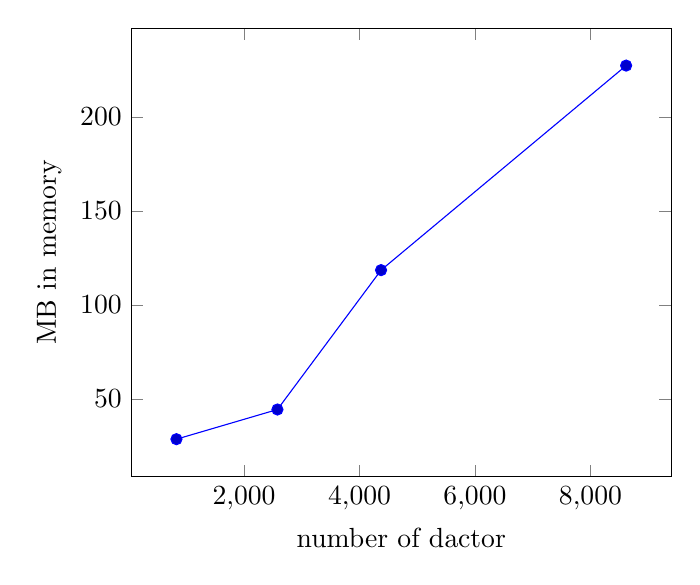
\begin{tikzpicture}
      \begin{axis}[xlabel=number of \glspl{dactor},ylabel=MB in memory]
        \addplot coordinates {
          (829,28.5)
          (2578,44.3)
          (4373,118.5)
          (8618,227.4)
        };
      \end{axis}
    \end{tikzpicture}
    \caption{Memory consumption as a function of the number of \glspl{dactor}}
    \label{fig:exp:dactors}
  \end{figure}


  \begin{figure}
    \centering
    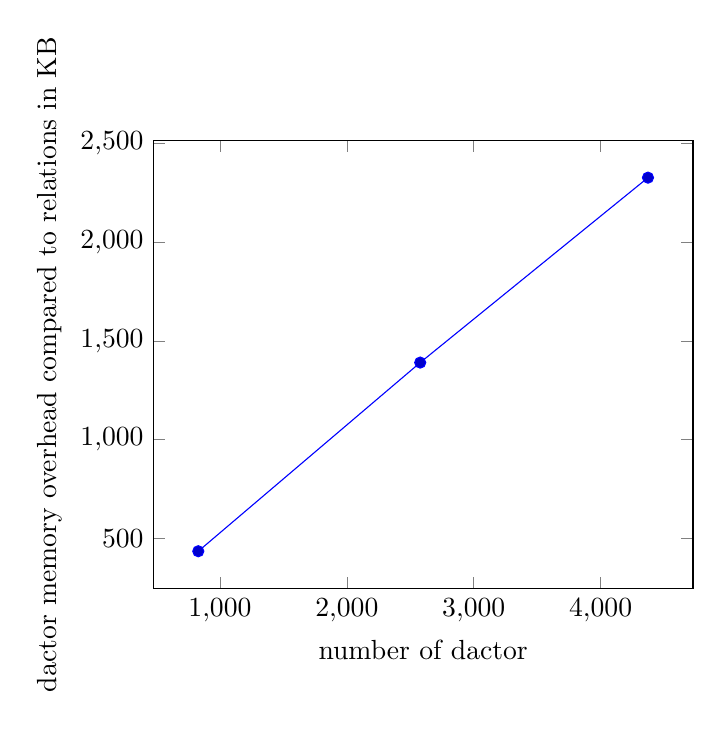
\begin{tikzpicture}
      \begin{axis}[xlabel=number of \glspl{dactor},ylabel=\gls{dactor} memory overhead compared to relations in KB]
        \addplot coordinates {
          (829,436)
          (2578,1390)
          (4373,2325)
        };
      \end{axis}
    \end{tikzpicture}
    \caption{Memory overhead of \glspl{dactor} as a function of the number of \glspl{dactor}}
    \label{fig:exp:dactoroverhead}
  \end{figure}

  \begin{figure}
    \centering
    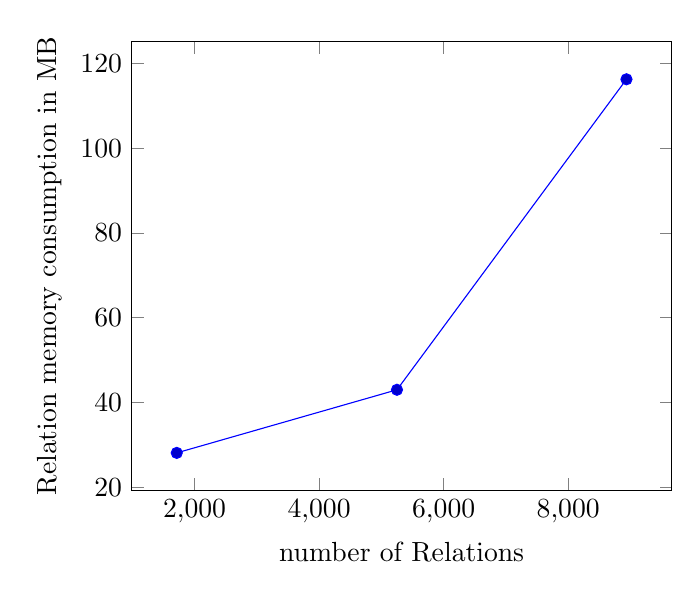
\begin{tikzpicture}
      \begin{axis}[xlabel=number of Relations,ylabel=Relation memory consumption in MB]
        \addplot coordinates {
          (1714,28.1)
          (5250,43.0)
          (8935,116.3)
        };
      \end{axis}
    \end{tikzpicture}
    \caption{Memory overhead of Relations as a function of the number of Relations}
    \label{fig:exp:relationoverhead}
  \end{figure}

\subsection{Discussion}
